%% Basierend auf einer TeXnicCenter-Vorlage von Tino Weinkauf.
%%%%%%%%%%%%%%%%%%%%%%%%%%%%%%%%%%%%%%%%%%%%%%%%%%%%%%%%%%%%%%

%%%%%%%%%%%%%%%%%%%%%%%%%%%%%%%%%%%%%%%%%%%%%%%%%%%%%%%%%%%%%
%% HEADER
%%%%%%%%%%%%%%%%%%%%%%%%%%%%%%%%%%%%%%%%%%%%%%%%%%%%%%%%%%%%%
\documentclass[a4paper,12pt]{report}
% Alternative Optionen:
%	Papiergr��e: a4paper / a5paper / b5paper / letterpaper / legalpaper / executivepaper
% Duplex: oneside / twoside
% Grundlegende Fontgr��en: 10pt / 11pt / 12pt


%% Deutsche Anpassungen %%%%%%%%%%%%%%%%%%%%%%%%%%%%%%%%%%%%%
%\usepackage[ngerman]{babel}
\usepackage[T1]{fontenc}
\usepackage[ansinew]{inputenc}

\usepackage{lmodern} %Type1-Schriftart f�r nicht-englische Texte


%% Packages f�r Grafiken & Abbildungen %%%%%%%%%%%%%%%%%%%%%%
\usepackage{graphicx} %%Zum Laden von Grafiken
%\usepackage{subfig} %%Teilabbildungen in einer Abbildung
%\usepackage{pst-all} %%PSTricks - nicht verwendbar mit pdfLaTeX

%% Beachten Sie:
%% Die Einbindung einer Grafik erfolgt mit \includegraphics{Dateiname}
%% bzw. �ber den Dialog im Einf�gen-Men�.
%% 
%% Im Modus "LaTeX => PDF" k�nnen Sie u.a. folgende Grafikformate verwenden:
%%   .jpg  .png  .pdf  .mps
%% 
%% In den Modi "LaTeX => DVI", "LaTeX => PS" und "LaTeX => PS => PDF"
%% k�nnen Sie u.a. folgende Grafikformate verwenden:
%%   .eps  .ps  .bmp  .pict  .pntg


%% Packages f�r Formeln %%%%%%%%%%%%%%%%%%%%%%%%%%%%%%%%%%%%%
\usepackage{amsmath}
\usepackage{amsthm}
\usepackage{amsfonts}

\usepackage[french]{babel}
\usepackage{fullpage}
\usepackage{eso-pic}
\usepackage{textcomp}
%\begin{center}
\usepackage{multirow}
\usepackage{cite}
%\end{center}
\usepackage{url} 
\usepackage{enumitem}
\usepackage{fullpage}
%\usepackage[top=3.0cm]{geometry}
\usepackage[top=2.5cm, left=2cm, right=2cm]{geometry}
\usepackage{titlesec}
\usepackage{setspace}
\usepackage{fancyhdr}
\usepackage[hidelinks]{hyperref}
\usepackage{float,caption}
\usepackage{listings}
\usepackage{xcolor}
\usepackage{color}

\definecolor{codegreen}{rgb}{0,0.6,0}
\definecolor{codegray}{rgb}{0.5,0.5,0.5}
\definecolor{codepurple}{rgb}{0.58,0,0.82}
\definecolor{backcolour}{rgb}{0.95,0.95,0.92}

\lstdefinelanguage{JavaScript}{
  keywords={break, case, catch, continue, debugger, default, delete, do, else, false, finally, for, function, if, in, instanceof, new, null, return, switch, this, throw, true, try, typeof, var, void, while, with},
  morecomment=[l]{//},
  morecomment=[s]{/*}{*/},
  morestring=[b]',
  morestring=[b]",
  ndkeywords={class, export, boolean, throw, implements, import, this},
  keywordstyle=\color{blue}\bfseries,
  ndkeywordstyle=\color{darkgray}\bfseries,
  identifierstyle=\color{black},
  commentstyle=\color{purple}\ttfamily,
  stringstyle=\color{red}\ttfamily,
  sensitive=true
}

\lstset{
   language=JavaScript,
   backgroundcolor=\color{lightgray},
   extendedchars=true,
   basicstyle=\footnotesize\ttfamily,
   showstringspaces=false,
   showspaces=false,
   numbers=left,
   numberstyle=\footnotesize,
   numbersep=9pt,
   tabsize=3,
   breaklines=true,
   showtabs=false,
   captionpos=b
}

\graphicspath{ {./images/} }



%% Zeilenabstand %%%%%%%%%%%%%%%%%%%%%%%%%%%%%%%%%%%%%%%%%%%%
%\usepackage{setspace}
%\singlespacing        %% 1-zeilig (Standard)
%\onehalfspacing       %% 1,5-zeilig
%\doublespacing        %% 2-zeilig


%% Andere Packages %%%%%%%%%%%%%%%%%%%%%%%%%%%%%%%%%%%%%%%%%%
%\usepackage{a4wide} %%Kleinere Seitenr�nder = mehr Text pro Zeile.
%\usepackage{fancyhdr} %%Fancy Kopf- und Fu�zeilen
%\usepackage{longtable} %%F�r Tabellen, die eine Seite �berschreiten


%%%%%%%%%%%%%%%%%%%%%%%%%%%%%%%%%%%%%%%%%%%%%%%%%%%%%%%%%%%%%
%% Anmerkungen
%%%%%%%%%%%%%%%%%%%%%%%%%%%%%%%%%%%%%%%%%%%%%%%%%%%%%%%%%%%%%
%
% Zu erledigen:
% 1. Passen Sie die Packages und deren Optionen an (siehe oben).
% 2. Wenn Sie wollen, erstellen Sie eine BibTeX-Datei
%    (z.B. 'literatur.bib').
% 3. Happy TeXing!
%
%%%%%%%%%%%%%%%%%%%%%%%%%%%%%%%%%%%%%%%%%%%%%%%%%%%%%%%%%%%%%


%%%%%%%%%%%%%%%%%%%%%%%%%%%%%%%%%%%%%%%%%%%%%%%%%%%%%%%%%%%%%
%% Optionen / Modifikationen
%%%%%%%%%%%%%%%%%%%%%%%%%%%%%%%%%%%%%%%%%%%%%%%%%%%%%%%%%%%%%

%\input{optionen} %Eine Datei 'optionen.tex' wird hierf�r ben�tigt.
%% ==> TeXnicCenter liefert m�gliche Optionendateien
%% ==> im Vorlagenarchiv mit (Datei | Neu von Vorlage...).


%%%%%%%%%%%%%%%%%%%%%%%%%%%%%%%%%%%%%%%%%%%%%%%%%%%%%%%%%%%%%
%% DOKUMENT
%%%%%%%%%%%%%%%%%%%%%%%%%%%%%%%%%%%%%%%%%%%%%%%%%%%%%%%%%%%%%

\newenvironment{dedication}
  {%\clearpage           % we want a new page          %% I commented this
   \thispagestyle{empty}% no header and footer
   % some space at the top
   \itshape             % the text is in italics
    \Large       % flush to the right margin
  }
  {\par % end the paragraph
   \vspace{\stretch{3}} % space at bottom is three times that at the top
   \clearpage           % finish off the page
  }
	
	
	\onehalfspacing
\setcounter{secnumdepth}{4}
\setcounter{tocdepth}{4}
\pagestyle{fancy}
\fancyhead[L]{\nouppercase\leftmark}
\fancyhead[R]{}
\titleformat{\paragraph}
{\normalfont\normalsize\bfseries}{\theparagraph}{1em}{}
\titlespacing*{\paragraph}
{0pt}{3.25ex plus 1ex minus .2ex}{1.5ex plus .2ex}

\geometry{headsep=1cm}

\newcommand{\HRule}{\rule{\linewidth}{0.5mm}}
\newcommand{\blap}[1]{\vbox to 0pt{#1\vss}}
\newcommand\AtUpperLeftCorner[3]{%
  \put(\LenToUnit{#1},\LenToUnit{\dimexpr\paperheight-#2}){\blap{#3}}%
}
\newcommand\AtUpperRightCorner[3]{%
  \put(\LenToUnit{\dimexpr\paperwidth-#1},\LenToUnit{\dimexpr\paperheight-#2}){\blap{\llap{#3}}}%
}

\begin{document}
%\pagestyle{empty} %%Keine Kopf-/Fusszeilen auf den ersten Seiten.
\begin{singlespace}

\begin{titlepage}
\pagenumbering{gobble}
    \enlargethispage{2cm}
 
    \AddToShipoutPicture{
       \AtUpperLeftCorner{1.5cm}{2.5cm}{
\includegraphics[width=2cm]{./../images/logo_iset_rades}}
      }
		\begin{center}
		\bf
		\begin{tabular}{c}
		\small
		Minist�re de l'Enseignement Sup�rieur et de la Recherche\\
		Scientifique\\
		Direction G�n�rale des Etudes Technologiques\\ \\
		Institut Sup�rieur des Etudes Technologiques de Rad�s\\ 
		D�partement Technologies de l'Informatique
		\end{tabular}
		\end{center}
		
		\vspace{2cm}
			
		
 
		\begin{center}
			\bf
			\Large
			\vspace{1.5cm}
			Rapport de
		\end{center}
		
		\begin{center}
		\bf
		\huge
			PROJET DE FIN D'ETUDES
		\end{center}
		
		\begin{center}
		\bf
			Pr�sent� en vue de l'obtention du dipl�me de
		\end{center}

		\begin{center}
		 \bf
			\large
			Master Professionnel en Business Intelligence
		\end{center}
		
		\begin{center}
		  \large
			\bf
			Parcours: MPBI \\ 
			\textbf{Insertion \& Employabilit�}
		\end{center}
		\begin{center}
			\bf
			\vspace{1.5cm}
			Elabor� par:\\
			Fedia Ghobghob Hatira
		\end{center}
		\begin{center}
			\bf
			\vspace{1cm}
			Encadr� par:\\
			Mme Nesrine Elleuch
		\end{center}
		\begin{center}
			\bf
			\vspace{1cm}
			Effectu� �:\\
			Entreprise: ISET Rad�s \\
			Encadrant: Mme Nesrine Elleuch
		\end{center}	
		\begin{center}
			\bf
			\vspace{1cm}
			P�riode: Fev - Juin 2022
		\end{center}	
		\begin{center}
			\bf
			\vspace{2cm}
			Ann�e Universitaire: 2021/2022
		\end{center}
			
\end{titlepage}
\ClearShipoutPicture

\end{singlespace}

\newpage
\begin{dedication}
\vspace{5.8cm}
	%\usefont{T1}{LobsterTwo-LF}{bx}{it}
		\begin{center}
		\large
			Du plus profond de mon c\oe{}ur, je d�die ce travail � tous ceux qui me sont chers,
		\end{center}
		
	\begin{center}
	   \Huge{ A mes chers parents }
	\end{center}
	\begin{center}
		\large{Aucune d�dicace ne saurait exprimer mon respect, mon amour �ternel et ma consid�ration pour les sacrifices que vous avez consentis pour mon instruction et mon bien-�tre.\\ Je vous remercie pour tout le soutien et l'amour que vous me portez depuis mon enfance et j'esp�re que vos b�n�dictions m'accompagneront pour toujours.\\
Que ce modeste travail soit l'exaucement de vos v\oe{}ux tant formul�s, le fruit de vos innombrables sacrifices. Puisse Dieu l'omnipr�sent, l'omnipuissant et l'omniscient, vous accorder sant�, bonheur et long�vit�.\\
 A mes tr�s chers fr�res et soeurs ainsi qu�� toute la famille. A mes amis et � tous mes proches pour leurs encouragements, leurs assistances et les soutiens inconditionnels. A tous les professeurs de l�ISET de Rad�s, plus particuli�rement � ceux du d�partement Informatique
} 
	\end{center}
	\begin{figure}[!h]
		\begin{flushright}
			
\includegraphics[width=50mm]{signatureelectronique}\\
			\normalsize{Fedia Ghobghob Hatira}
		\end{flushright}
	\end{figure}
\end{dedication}

\newpage
\begin{center}
		\bf
		\Huge
		REMERCIEMENTS \\
\end{center}
\vspace{1cm}
	\begin{dedication}
    %\usefont{T1}{LobsterTwo-LF}{bx}{it}
		\begin{center}
		\large
			Il m�est offert ici par quelques lignes la possibilit� de remercier les personnes qui ont
contribu� � faire de ce projet une r�ussite au sein de l'Institut Sup�rieur des Etudes 
Technologique de Rad�s, un bon stage.

Je tiens � remercier et � exprimer ma profonde gratitude � notre ch�re professeure et encadrante 
Mme Nesrine Elleuch pour son suivi, accompagnement, son �norme soutien et ses conseils 
qu'elle  m'a prodigu�s tout au long de ce stage.

L�occasion m�est donn�e ici de remercier aussi mes camarades de promotion universitaire
pour leur esprit de coh�sion et de partage qui ont contribu� � rendre brillante et enrichissante
cette ann�e universitaire.	

\end{center}
\end{dedication}	
\pagenumbering{roman}
\renewcommand{\contentsname}{Sommaire}
\tableofcontents	
\listoffigures
\listoftables
\newpage
\pagenumbering{arabic}		

\chapter{Contexte du projet}
\section{Introduction}
L��tude pr�alable constitue une �tape primordiale dans le processus de la r�alisation d�un projet.

Dans ce chapitre, nous pr�sentons l�organisme d�accueil � savoir l�Institut Sup�rieur des Etudes Technologique de Rades (ISET Rades) au sein duquel s�est d�roul� notre projet, Nous pr�senterons par la suite le cadre g�n�ral du projet, puis un diagnostic de l�existant pour d�gager les insuffisances et proposer les orientations de notre future solution.

Nous expliquerons, enfin, le planning de notre projet

\subsection{Pr�sentation de l�organisme d�accueil}

\subsubsection{Cr�ation}
l�ISET Rad�s (Institut sup�rieur des �tudes technologiques de Rad�s) cr�� par la loi 51-92 du 18 mai 1992; est un institut universitaire tunisien rattach� � la direction g�n�rale des �tudes technologiques. Plac� sous la tutelle du minist�re de l�Enseignement sup�rieur et de la Recherche scientifique et g�r� par la direction g�n�rale,il propose une formation initiale dipl�mante, des formations continues en lien avec les besoins des entreprises, un centre de ressources technologiques, un p�le de comp�tence et une p�pini�re d�entreprises. L�enseignement y est assur� en grande partie par des enseignants du corps des technologues.

\subsubsection{Mission}
ISET-Rad�s est une institution d�enseignement Sup�rieur tunisienne formant des �tudiants en vue de l�obtention du dipl�me de licence appliqu�e et de mast�re professionnel dans plusieurs domaines. Il assure la formation selon la r�forme LMD du syst�me de l�enseignement sup�rieur tunisien au sein des d�partements suivants : g�nie m�canique, g�nie civil, g�nie �lectrique, technologies de l�informatique et des sciences �conomiques et de gestion.\\
La mission de l�ISET de Rad�s est de � fournir au march� de l�emploi des cadres moyens qualifi�s aussi bien dans les secteurs secondaires que tertiaire, de promouvoir le recyclage et la formation continue au profit des cadres exer�ant dans les entreprises (formation dipl�mante en cours de soir, formation sp�cifique et ponctuelle ) et de mettre en place un partenariat avec les entreprises et les organisations professionnelle � travers la participation des professionnels � la formation et � l�encadrement des �tudiants ainsi que la r�alisation conjointe de programme de recherche appliqu�e et de transfert de technologie �.

\subsubsection{Historique}
L�Institut Sup�rieur des Etudes Technologiques de Rad�s, fleuron du r�seau des ISET et porte drapeau de la formation technologique en Tunisie, a constitu� depuis sa cr�ation en septembre 1995, le principal pourvoyeur du march� de l�emploi en techniciens sup�rieurs aussi bien dans le secteur industriel que dans le secteur des services. En effet, la localisation de l�ISET de Rad�s dans l�une des r�gions � plus forte concentration industrielle du pays, la r�gion de Ben Arous, son int�gration dans une zone logistique comprenant le plus grand port tunisien et sa proximit� des plus grands p�les de commerce et de services de Tunis ville, ont permis � l�institut de conforter sa vocation r�gionale et d�assurer une responsabilit� grandissante vis-�-vis de ses partenaires professionnels.\\
Tout au long de ces 30 ans d�existence l�ISET de Rad�s a �t� pr�curseur en termes d�innovation p�dagogique et d�ouverture sur l�environnement professionnel. Il a �t� souvent la sc�ne de pr�dilection des exp�riences pilotes touchant le r�seau des ISET.\\

A ce titre l�ISET de Rad�s a lanc� depuis 2003 l�exp�rience pilote de l�enseignement � distance en Tunisie en collaboration avec l�UVT (d�partements de Gestion, de techniques de commercialisation et de commerce international), il a �t� le premier � d�crocher un financement dans le cadre du projet d�appui � la qualit� de l�enseignement sup�rieur PAQ (au profit du d�partement de G�nie M�canique, ann�e 2007), et a �galement mis en �uvre la m�me ann�es cinq licences co-construites r�pondant aux besoins imm�diats du tissu industriel (une licence co-construite en grande distribution avec la f�d�ration des services, deux licences co-construites en supervision et suivi des chantiers de travaux publics et en supervision et suivi des travaux de b�timents avec la f�d�ration des entrepreneurs de b�timents et de travaux publics, et deux autres licences co-construites en essais �lectriques et �lectroniques et en syst�mes �lectroniques de s�curit� avec la f�d�ration des �lectriciens FEDELEC).\\

En outre l�ISET de Rad�s a d�croch� le prix de l�innovation technologique par la cr�ation du Centre de Ressources Technologiques en CFAO, mis en place depuis 2005 dans le cadre de la coop�ration Tuniso-Fran�aise (Projet de coop�ration : Appui au d�veloppement de l�enseignement Technologique en Tunisie). Un centre qui se veut un organe de transfert de technologie et d�appui aux entreprises industrielles pour garantir la qualit� et les performances indispensables en vue de gagner le pari de la comp�titivit�.\\

En septembre 2008 ISET de Rad�s a int�gr� le syst�me LMD avec six licences appliqu�es en G�nie M�canique, en G�nie Electrique, en G�nie Civil, en Technologies de l�Informatique, en Administration des Affaires et en Marketing d�bouchant sur 21 parcours permettant la formation de licenci�s polyvalents capables de s�adapter aux exigences du march� de l�emploi. Ces licences ont �t� enrichies en 2014 par une nouvelle fili�re prometteuse, celle de Finance islamique et en arrivant � ce jour l�ISET atteint 53 parcours.

\subsubsection{Ouverture sur l�environnement et convention}
Dans le cadre de sa mission d�ouverture sur l�environnement socio-�conomique. L�ISET est li�e � plusieurs entreprises tunisiennes et internationales par des conventions de partenariat couvrant des contrats de recherche ou des contrats de formation continue. Aussi partenariat avec les entreprises et la soci�t� civile pour une meilleure visibilit� de l�ISET et des profils des dipl�m�s.\\

\begin{itemize}
	\item Participation d�un bon nombre de professionnels issues des milieux industriel et �conomique � l�enseignement des �tudiants de l�\textbf{ISET de Rad�s};
	\item Accueil des �tudiants de l�ISET de Rad�s au sein des entreprises en stages et en projets de fin d��tudes :
	\begin{itemize}
		\item 2000 � 2400 stages au sein des entreprises sont affect�s chaque ann�e depuis 1999.
		\item 400 � 500 projets de fin d��tudes � caract�re professionnel sont aussi propos�s chaque ann�e par les industriels pour les �tudiants du niveau terminal de l�\begin{bf}ISET Rad�s\end{bf}, et encadr�s conjointement par un enseignant de l�ISET et un responsable et l�entreprise.
	\end{itemize}
	\item Participation des industriels aux diff�rentes manifestations et expositions scientifiques et technologiques organis�es par l�\textbf{ISET de Rad�s};
	\item Participation de personnalit�s professionnelles au conseil scientifique et technologique et au comit� de direction de l�\textbf{ISET Rad�s};
	\item Participation � la d�finition des programmes des enseignements ;
\end{itemize}

La maturation progressive de l�institution associ�e � l�exp�rience et la comp�tence de ses enseignants permettant d�assurer une formation rigoureuse, l�importance des moyens et ressources technologiques d�une institution en pleine mutation qualitative et l��ventualit� de cr�ation de p�les de comp�tences � travers une vague de certification des enseignants permanents et des �tudiants. Par ailleurs, sa strat�gie s�articule sur le processus de certification de l��cole en mettant en �uvre l�SMQ aux termes de l�ISO 9001 en vue de l�accr�ditation de l�institut pr�vue � la lumi�re de l�ann�e universitaire 2021/2022.\\

En l�occurrence, les �tudiants en particulier b�n�ficient d�un panier de certification (TOEIC, CISCO, C2i, Solid Works,  LabView �) leurs permettant une int�gration meilleure dans le secteur professionnel. En outre, l�institut est bien �quip� pour r�pondre d�une mani�re satisfaisante aux exigences de la formation pratique (travaux pratiques) dans les diff�rents parcours d�j� habilit�s. Les �l�ments sus indiqu�s constituent des signes prometteurs en vue d�une revalorisation du statut de notre institut pour une r�ponse plus pointue aux besoins des professionnels aussi bien en cadres moyens (licence appliqu�es) qu�en cadres sup�rieurs (masters professionnels).

\subsubsection{Les services de l�ISET.}
L�organisation de l�ISET est pr�sent�e sous forme de l�administration qui capitalise plusieurs services
Notamment :
\begin{itemize}
	\item Services des �tudes et de Stage.
    \item Secr�tariat G�n�ral.
    \item Conseil Scientifique. 
    \item Services Scolarit�.
    \item Service Examen.
    \item Service Financier et Enseignant.
    \item Service de Resource Humain.
    \item Biblioth�que.
    \item Service de maintenance.
    \item Les d�partements.
    \item Bureau d�Ordre.
    \item Service partenarial, relations avec l'environnement et formation continue.
    \item Service de Tirage.
    \item L�infirmerie.
    \item Bureau de conseil, d'assistance et d'intervention psychologique.
\end{itemize}

\subsubsection{Principaux Services en relation avec les �tudiants}
\begin{itemize}
	\item \begin{bf}Service Scolarit�\end{bf}: qui a pour r�le la pr�paration de l�inscription notamment :
	\begin{enumerate}
		\item faire l�inscription des nouveaux (nouveau bachelier) et anciens �tudiants et les affecter dans des groupes de classe;
		\item fournir les attestations des inscriptions, les attestations de pr�sence, les attestations de d�part, les attestations de retrait et toute autres attestations demand� par l'�tudiant;
		\item Pr�paration et remise des dipl�mes;
	\end{enumerate}
	\item  \textbf{Service de stages}:  a pour r�le de faire le suivi des notes de stages d�initiation, perfectionnement ou de PFE, les partager sur la plateforme \begin{bf}DIDOSOFT\end{bf} pour qu�elle soit visible pour les �tudiants et le service Examen.
	\item \begin{bf}Service Examen\end{bf}: qui a pour r�le la pr�paration des examens et suivi des r�sultats notamment:
	\begin{enumerate}
		\item recueille les notes des �tudiants de diff�rents d�partements � travers le syst�me DIDOSOFT ou manuellement;
		\item saisir les notes, calcul les moyennes et faire sortir les PVs;
		\item fournir les relev�s et les attestations de r�ussites;
	\end{enumerate}
	\item \begin{bf}D�partements\end{bf} qui jouent un r�le p�dagogique avec les �tudiants.
	\item \begin{bf}Bureau de conseil, d'assistance et d'intervention psychologique\end{bf}.
	\item \begin{bf}l'infirmerie\end{bf}
\end{itemize}

\subsection{Cadre du projet}
Notre projet s�inscrit dans le cadre d�un projet de fin d��tudes pour l�obtention du Mast�re Professionnel en Business Intelligence. Le but principal de l�institut est de garder un historique complet sur leurs �tudiants m�me faire un suivie toute au long de leurs cursus scolaires dans le but de conna�tre quelles sont les parcours et les sp�cialit�s qui ont un bon pourcentage de r�ussite, Aussi un suivie concernant les conventions fournit � l�ISET. Et ce afin d�y rem�dier et assurer l�am�lioration du contenue de la formation.

\begin{large}Motivation\end{large}
En �tant qu��tudiante en master Business Intelligence, � l�ISET Rades, j�ai voulu contribuer � l��volution de notre �tablissement en cr�ant des tableaux de bord permettant de piloter certaines des activit�s de l�institut. En effet :\\
L�ISET souffre du manque d�outils d�cisionnels qui fournissent les diff�rents �l�ments d�information n�cessaires pour avoir une vision historis��e des diff�rentes donn�es et permettre d��ventuelles prises de d�cision.

\subsection{Description du contexte du projet}
Cette section a pour objectif de pr�senter le contexte du projet, de poser la probl�matique et d��tudier l�existant afin d�exposer ma solution. 

\subsubsection{Probl�matique}
La d�cision n�cessite une mati�re premi�re : la donn�e ou l�information. Si l'information est incompl�te, floue, impr�cise..., probablement, les d�cisions seront approximatives, inadapt�es, voire fatales ; par contre si l'information est exacte, compl�te et pertinente, les d�cisions ont davantage de chances d'avoir une efficacit� garantie. Justement, le manque de cette mati�re premi�re sous forme d�information utile ou bien la difficult� de la faire ressortir, constitue aujourd�hui, une vraie probl�matique pour les responsables au sein de l�ISET pour l��laboration des rapports de gestion, l��dition des graphes et statistiques et les probl�mes de prise de d�cisions en g�n�ral.

\subsubsection{�tude de l�existant}
Dans cette section nous pr�sentons notre projet en commen�ant par une �tude de l�existant en identifiant l�environnement logiciel dans lequel notre �tude va �tre men�e et analyser les structures des donn�es du logiciels de gestion de scolarit� et de note de l�ISET, ensuite nous allons enchainer par la solution propos�e et la m�thodologie adopt�e pour r�ussir notre mission.

\subsubsection{Identification de l�environnement}
En analysant la situation actuelle, on a pu distinguer deux syst�mes sources qui sont :\\
\begin{bf}SALIMA\end{bf} (Syst�me d'Administration des LIcences et MAst�res), et un autre logiciel nomm� `GestionNote` \& `Scolarit�` sp�cialement pour la gestion d�inscription et gestion de note du parcours mast�res. Ce logiciel est �labor� par un enseignant universitaire.\\
``SALIMA`` comporte trois axes. \\
\begin{itemize}
	\item Le premier est relatif � la gestion p�dagogique des fili�res scientifiques dans les divers �tablissements universitaires en ce qui concerne la d�finition des contenus de la formation et le suivi de leur application.
	\item Le second concerne la gestion des services universitaires et des affaires estudiantines telles que l'inscription universitaire, le syst�me de notation, la carte d'�tudiant, la carte de biblioth�que, le relev� des notes ainsi que les attestations de r�ussite et les dipl�mes.
	\item Le troisi�me axe porte sur la gestion des examens universitaires.
\end{itemize}
Le ministre a pr�cis� que l'application "SALIMA" intervient en vue de faciliter la gestion des �tablissements universitaires conform�ment au r�gime \begin{bf}LMD\end[bf} (Licence Mast�re Doctorat).\\

Mais comme tout syst�me peut avoir des avantages et des inconv�nients, \begin{bf}SALIMA\end{bf} et l�autre logiciel ont les lacunes suivantes :
\begin{itemize}
	\item Pas de dictionnaire de donn�es.
	\item Pas de tableau de bord.
    \item Format des fichiers incoh�rent. 
    \item Pas de tra�abilit� des donn�es.
\end{itemize}

\subsubsection{Solution propos�e}
C�est pour �a nous proposons la mise en place d�une solution BI qui couvre l�ensemble de processus allant de l�historisation des donn�es jusqu�� la diffusion d�une vue globale sur un tableau de bord clair permettant ainsi une analyse pertinente et pr�cise.\\

La d�marche de cette solution est planifi�e en 3 �tapes :
\begin{itemize}
	\item La premi�re �tape consiste � rassembler les donn�es � partir du syst�me SALIMA et le syst�me du parcours mast�re concernant les �tudiants encore pr�sents, � les traiter et � les stocker, l�objectif est de garder un historique complet des �tudiants. Ainsi que le rassemblement des donn�es concernant les conventions de l�ISET. 
	\item La deuxi�me volet porte sur la production des rapports destin�s aux d�cideurs de l�institut pour avoir une vision d�taill�e et explicite sur les �tudiants en question.
\end{itemize}

Dans les tableaux de bord, nous devons pr�senter des indicateurs qui permettront de suivre :
\begin{enumerate}
	\item Les �tudiants au sein de l�ISET d�s leurs inscriptions jusqu�aux obtention du dipl�me.
	\item Les conventions, leurs dur�es, les th�mes et les partenaires qui ont sign� plus grand nombre convention avec l�ISET.
\end{enumerate}

Ces indicateurs sont class�s dans le tableau suivant qui nous a permis de recenser les diff�rents rapports dont les d�cideurs ont besoin :
\begin{table}[!h]
	\centering
		\begin{tabular}{|p{4cm}|p{3cm}|p{9cm}|}
        	\hline
        	\begin{bf}Rapport\end{bf} & \begin{bf}Cat�gorie\end{bf} & \begin{bf}Description\end{bf} \\ 
        	\hline
        	Nombre des �tudiants qui ont abandonn�s & Histogramme & Cet histogramme repr�sente le nombre des �tudiants qui ont abandonn� leur parcours sur l'axe y et les diff�rents parcours sur l�axe x\\ 
        	\hline
         	Nombre des �tudiants dipl�m�s par d�partement  & Histogramme & Cet histogramme montre le nombre des �tudiants qui ont obtenu leurs dipl�mes, soit dans la s�rie licence ou master : l�axe y repr�sente le nombre des �tudiants, l�axe x repr�sente le type du dipl�me obtenu par l��tudiant (licence, master). \\ 
        	\hline
         	Nombre des �tudiants par d�partement & Histogramme & Cet histogramme permet aux d�cideurs de visualiser les effectifs des �tudiants par d�partement, sur l�axe y on trouve le nombre des �tudiants, sur l�axe x les diff�rents d�partements.\\ 
        	\hline
         	Nombre des �tudiants par observation & Histogramme & Cet histogramme montre le nombre d��tudiants selon leur observation (Admis ou Redouble)\\ 
        	\hline
         	Nombre des �tudiants par Sp�cialit� & Histogramme & Cet histogramme permet de visualiser les effectifs des �tudiants par sp�cialit�, sur l�axe y on trouve le nombre des �tudiants et sur l�axe x les diff�rentes sp�cialit�s.\\ 
        	\hline
         	Effectif des �tudiants par type dipl�me  & Camembert & Ce camembert affiche l�effectif des �tudiants selon leurs dipl�mes (licence, master).\\ 
        	\hline
        	Effectif des �tudiants par type d�partement & Camembert & Ce camembert affiche l�effectif des �tudiants par d�partement\\ 
        	\hline
        	Nombre des �tudiants par gouvernorat & Carte & Ce rapport sous forme d�une carte g�ographique expose le nombre des �tudiants selon leurs gouvernorat d�origine.\\ 
        	\hline
        	Nombre des �tudiants par genre & Table & Cette table affiche le nombre des �tudiants selon leur genre (Homme ou Femme)\\ 
        	\hline
        	Nombre des �tudiants par �tat & Table & Cette table affiche le nombre des �tudiants selon leurs �tat (Confirm�, Retrait, D�part)\\
        	\hline
        	Taux de R�ussite par d�partement & Table & Cette table affiche le pourcentage de r�ussite des �tudiants par d�partement\\
        	\hline
        	Taux de R�ussite par sp�cialit� &  Table & Cette table affiche le pourcentage de r�ussite des �tudiants par sp�cialit�\\
        	\hline
        	Nombre de convention par type & Histogramme & Cet histogramme repr�sente le nombre des conventions par type \\
        	\hline
        	Nombre de convention par th�me & Histogramme & Cet histogramme repr�sente le nombre des conventions par th�me \\
            \hline
            Dur�e moyenne des conventions & Table & Cette table affiche la dur�e moyenne des conventions par type ou th�me \\
            \hline
            Nombre de partenaires & Table & Cette table affiche le nombre de partenaire qui ont sign� une convention \\
            \hline
		\end{tabular}
	\caption{Tableau r�capitulatif des diff�rents rapports requis}
	\label{Tableau r�capitulatif des diff�rents rapports requis}
\end{table}
\newpage
\subsection{Contrainte du projet}
Un projet d�cisionnel peut subir des difficult�s il est n�cessaire d��valuer les facteurs qui peuvent ralentir le d�roulement du projet. Apr�s l��tude de l�existant on s�est oppos� � une multitude de probl�mes et difficult�s majeures qui nous ont retard�s dans notre d�marche.\\
La liste suivante contient une liste non exhaustive des obstacles et des probl�mes les plus importants : 

\begin{itemize}
	\item Manque d�historisation des donn�es;
    \item Manque de Bases de donn�es ;
    \item Donn�es non structur�es ;
    \item Tables non r�f�renc�es (pas de relations entre les tables) ; 
    \item Champs de tables non renseign�s (vide) ou partiellement renseign�s ;
    \item Champs remplis de mani�re erron�e ;
    \item Manque de donn�es pour faire ex�cuter les requ�tes.
    \item Champs redondants (M�me champs retrouv� plusieurs fois dans la base de donn�es) 
\end{itemize}

\subsection{Cycle de vie d�un projet d�cisionnel}
L�impl�mentation d�un syst�me Business Intelligence/Intelligence d�affaires doit �tre pilot�e par une m�thodologie globale. Une m�thodologie qui diff�re des m�thodologies de d�veloppement des syst�mes transactionnels.\\

Pour garantir l�aspect fonctionnel du projet et avoir des r�sultats rapides nous suivrons une m�thodologie par cycles it�ratifs de `Ralph Kimball`. Cette m�thode est illustr�e par le sch�ma suivant :
\begin{figure}
   \begin{center}
		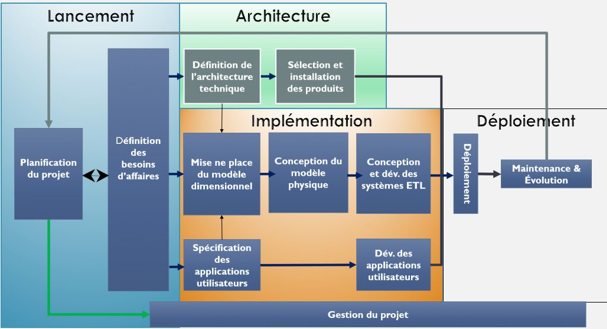
\includegraphics{cycleDeVieProjetDecisionnel}
	\end{center}
    \caption{Cycle de vie d�un projet decisionnel selon RALPH KIMBALL}
	\label{Cycle de vie d�un projet decisionnel selon RALPH KIMBALL}
\end{figure}

Pour en savoir plus pour chaque phase et chaque �tape du projet je vais pr�senter les diff�rentes phases dans l�ordre :

\subsubsection{Planification}
La planification aborde la d�finition et l��tendue du projet de l�entrep�t, elle se focalise sur les besoins en termes de ressources et de niveau de qualification, coupl�es aux affectations des t�ches, � leurs dur�es et � leur s�quencement.

\subsubsection{La d�finition des besoins de l�entreprise}
Comprendre les attentes du client et de ses exigences non �nonc�es, poser les bonnes questions et tirer l�information du client. Ce niveau va pr�parer le terrain du travail en termes de 3 trajectoires ; La technologie, le mod�le et l�interface client.

\subsubsection{Conception du mod�le physique }
La conception physique d�une base de donn�es d�finit les structures n�cessaires pour l�impl�mentation du mod�le dimensionnel.

\subsubsection{Mod�lisation multidimensionnelle}
Elaboration du mod�le multidimensionnel des donn�es : faits et dimensions et la r�alisation des maquettes de la solution d�cisionnelle propos�e.

\subsubsection{Conception et d�veloppement des �l�ments de la zone de pr�paration des donn�es }

Concevoir et d�velopper les �tapes d�ETL qui vont r�sulter des donn�es nettoy�es et atomiques alimentant notre magasin de donn�es.

\subsubsection{D�finition de l�architecture technique}
Cette �tape d�finit la vision globale de l�architecture technique � mettre en oeuvre. Elle n�cessite la prise en compte de trois facteurs : Les besoins ; L�environnement existant et les orientations techniques strat�giques planifi�es.

\subsubsection{S�lection et installation des outils}
R�aliser une �tude comparative des outils pour chaque phase de la cha�ne d�cisionnelle.

\subsubsection{Conception de l�application BI}
Il s�agit de d�finir une s�rie d�applications standard destin�es aux utilisateurs finaux. Les sp�cifications de l�application d�crivent les maquettes d��tats, les crit�res de s�lection laiss�s � l�utilisateur et les calculs n�cessaires.


\subsubsection{D�veloppement de l�application utilisateur}
D�velopper les tableaux de bord et indicateurs de performance sp�cifique pour chaque utilisateur. 

\subsubsection{D�ploiement}
Int�grer apr�s validation et test, l�application au sein de l�organisme. 


\subsubsection{Maintenance et croissance}
Il faut s�assurer de fournir un service de support et de formation continue. Il est �galement important de mesurer p�riodiquement l��volution et la croissance des performances de l�entrep�t de donn�es au sein de l�entreprise.

\subsubsection{Gestion du projet}

Garantir le bon d�roulement des activit�s du cycle de vie dimensionnel, contr�ler l��tat d�avancement du projet et enfin d�tecter et r�soudre des probl�mes. Dans l�obligation de trouver une m�thode qui englobe toutes les phases du projet permettant de satisfaire le client dans les plus brefs d�lais, nous allons utiliser la m�thodologie � Ralph KIMBALL � pour notre projet vue qu�elle s�adapte au mieux � nos besoins en termes de comp�tences, de temps, de co�t et d�exigence en ce qui concerne l�int�gration de donn�es.

\subsection{Planification du projet}
Le d�veloppement de tout projet n�cessite une phase de planification qui permet de d�finir les t�ches � r�aliser, ma�triser les risques et rendre compte de l��tat d�avancement du projet. Dans le but d�une meilleure organisation du projet et gestion efficace des d�lais disponibles, j�ai pr�sent� sous forme de diagramme de GANTT qui illustre cet ordonnancement.

\begin{figure}[!h]
	\begin{center}
		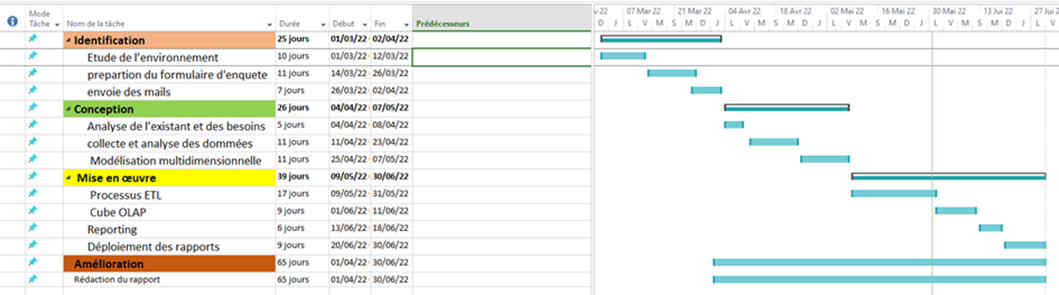
\includegraphics[]{diagrammeDeGant}
	\end{center}
	\caption{Diagramme de Gant}
	\label{Diagramme de Gant}
\end{figure}

\section{Conclusion}

Ce premier chapitre a fait l�objet d�une pr�sentation de l�existant, le cadrage du projet par l��laboration de sa probl�matique et les diff�rents objectifs.\\

A la fin de ce chapitre j�ai sp�cifi� un cycle de vie d�cisionnel standardis� assurant la r�alisation du projet ainsi que la planification.



\chapter{Notion Th�orique}
\section{Introduction}

Toutes les entreprises du monde poss�dent plus ou moins d'�normes quantit�s de donn�es. Ces informations proviennent de sources internes (g�n�r�es par le syst�me d'exploitation dans ses activit�s quotidiennes) ou de sources externes (web, fichiers plats, etc.)\\

Cette surabondance des donn�es d�une part, et les limites des syst�mes op�rationnels pour exploiter cette quantit� de donn�es � des fins d�analyse d�une autre part, ont conduit et pousser les entreprises � tourner vers une nouvelle �re informatique dite d�cisionnelle (Business Intelligence).\\

L�informatique d�cisionnelle, �galement Business Intelligence ou BI en anglais, d�signe les moyens, les m�thodes et les outils qui apportent des solutions en vue d�offrir une aide � la d�cision aux professionnels afin de leurs permettre d�avoir une vue d�ensemble sur l�activit� de l�entreprise et de leurs permettre de prendre des d�cisions plus avis�es � travers des tableaux de bord de suivi et des analyses.\\

\section{Les syst�mes d�cisionnels (Business Intelligence)}

La Business Intelligence d�signe les moyens, les outils et les m�thodes qui permettent de collecter, consolider, mod�liser et restituer les donn�es d'une entreprise en vue de fournir une aide � la d�cision aux managers. \\
Le terme fran�ais est � Informatique D�cisionnelle �. Une application de ce genre ex�cute la capture, l�analyse et le stockage de donn�es provenant de plusieurs sources h�t�rog�nes qui peuvent �tre des Enterprise Ressource Planning (ERP), des bases de donn�es ou d�autres entrep�ts de donn�es. 
Traditionnellement, un entrep�t de donn�es est utilis� comme source d�information par les d�cisionnaires. La Business Intelligence s�ins�re dans l�architecture du syst�me d�information d�une entreprise.\\
Avec Business Intelligence, nous comprenons les applications Business Intelligence. Cependant, le terme � business intelligence � ne fait pas directement r�f�rence � des outils informatiques, mais � ce que l'on fait avec ces outils afin d'effectuer des analyses pouss�es sur des objets pr�alablement identifi�s. Cette analyse peut �tre �tablie pour l'ensemble de l'entreprise, pour un d�partement ou une division sp�cifique, ou m�me pour un projet sp�cifique.\\
Pour pouvoir obtenir une vue compl�te des objets analytiques de haut niveau, les applications d'informatique d�cisionnelle utilisent des entrep�ts de donn�es comme sources d'informations. La t�che principale d'un entrep�t de donn�es est de filtrer, recouper et recat�goriser les informations pour fournir un g�n�rateur d'analyse de donn�es au niveau mondial. C'est-�-dire des donn�es pertinentes directement li�es � l'objet analys�. Dans la plupart des cas, ces donn�es proviennent de bases de donn�es relationnelles. Un entrep�t de donn�es est un clone de donn�es existantes au niveau op�rationnel d'une entreprise en pr�paration de probl�mes d'analyse et de performance. Les images des situations de l'entreprise ou les r�sultats produits par les g�n�rateurs d'analyses sont pr�sent�s sous forme de rapports statistiques ou sous forme de tableaux de bord d�cisionnels. Ces informations sont utilis�es pour v�rifier l�alignement de la strat�gie de l�entreprise et assister la direction de l�organisme, d�o� le nom d�informatique d�cisionnelle.

\begin{figure}[!h]
	\begin{center}
		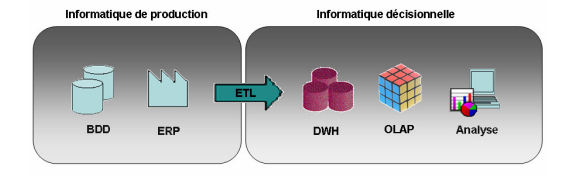
\includegraphics[]{passageABI}
	\end{center}
	\caption{Le passage de l'informatique de production � la l'informatique d\'ecisionnelle}
	\label{Le passage de l`informatique de production � la l`informatique d\'ecisionnelle}
\end{figure}

Le passage de l�informatique de production � l�informatique d�cisionnelle se fait par un Extract Transform Load (ETL). Les sources de donn�es les plus utilis�es dans ce genre de transaction sont les bases de donn�es. Les informations contenues dans la source de donn�es sont trait�es puis stock�es dans un entrep�t de donn�es. Les donn�es gard�es dans l�entrep�t de donn�es sont dans l��tat de consultation, et sont sujettes � l�analyse multidimensionnelle (OnLine Analytical Processing OLAP). Le r�sultat produit par l�analyse multidimensionnelle est appel� � cube �. Les cubes d�information sont trait�s par les g�n�rateurs d�analyse pour produire les reports demand�s. \cite{ref1}

\subsection{Les avantages d�une solution BI}
Sans aucun doute, le terme "BI" est devenu l'un des mots � la mode les plus utilis�s dans le monde du business. Les nouvelles solutions propos�es sont faciles � utiliser avec une interface ergonomique simple. Par contre, la question qu'il faut se poser est : "Est-ce que mon entreprise a vraiment besoin d'une solution BI ?". Si la r�ponse est oui : "Comment cela affecte-t-il mes d�cisions au sein de l'entreprise ?".\\
Voil� les b�n�fices apport�s couramment, en impl�mentant une solution BI au sein d�une organisation : 
\begin{itemize}
	\item Rapidit� de la prise de d�cision fond�e sur des faits.
    \item Am�liorer la visibilit� sur les chiffres, les �carts et les anomalies. 
    \item La combinaison de plusieurs sources de donn�es (ERP, syst�mes comptable, feuilles de calcul, des budgets �).
    \item La pr�sentation uniforme d�informations fiables pour les membres de l�organisation.
    \item L�automatisation permettant l�acc�l�ration de la collecte et de la diffusion de l�information. 
    \item La performance dans le calcul d�agr�gats sur de gros volume de donn�es.
    \item La prise de d�cision gr�ce � des indicateurs pertinents et � une structure coh�rente des informations. 
    \item L�aide � nettoyer les donn�es pr�sentes dans diff�rents logiciels. 
    \item L�anticipation des �v�nements et la projection dans l�avenir.
    \item Elaboration des rapports n�cessaires au bon moment, � tous les niveaux organisationnels, et dans les meilleurs formats possibles.
\end{itemize}


\subsection{Les domaines d�utilisation de la BI}
La \textbf{BI} est utilis�e dans plusieurs domaines nous citerons :
\begin{itemize}
	\item Finance, avec le reporting financiers et budg�taires. 
    \item Vente et commercial, avec l�analyse de points de vente, l�analyse de la profitabilit�.
    \item Marketing, avec la segmentation clients, les analyses comportementales. 
    \item Logistique, avec l�optimisation de la gestion de stock, le suivi des livraisons. 
    \item Ressources humaines, avec l�optimisation de l�allocation des ressources.
\end{itemize} 

\section{D�cisionnel vs transactionnel (OLAP vs OLTP)}
Les syst�mes informatiques peuvent se subdiviser en deux cat�gories : les syst�mes transactionnels OLTP (Online Transaction Processing) et les syst�mes analytiques OLAP (OnLine Analytical Processing).
\begin{itemize}
	\item Les syst�mes OLTP sont d�di�s aux m�tiers de l�entreprise pour les assister dans leurs t�ches de gestion quotidiennes et donc directement op�rationnels. Le mode de travail est transactionnel. L�objectif est de pouvoir ins�rer, modifier et interroger rapidement et en s�curit� la base. Ces actions doivent pourvoir �tre effectu�es tr�s rapidement par de nombreux utilisateurs simultan�ment. Il est propos� essentiellement pour les applications g�rant des op�rations commerciales comme les op�rations bancaires, ou l�achat de bien divers. \cite{ref3}
	\item Les syst�mes OLAP sont d�di�s au management de l�entreprise pour l�aider au pilotage de l�activit�. C�est un outil de reporting dont la couche d�analyse permet de g�n�rer des r�sultats en fonction du contenu d�un entrep�t de donn�es. Les programmes consultent une quantit� importante de donn�es pour proc�der � des analyses. Les objectifs principaux sont : regrouper, organiser des informations provenant de sources diverses, les int�grer et les stocker pour permettre � l�utilisateur de retrouver et analyser l�information facilement et rapidement. \cite{ref3}
\end{itemize}

Bien que les syst�mes d�informations \textbf{OLTP} et \textbf{OLAP} aient le point commun de regrouper les donn�es de l�entreprise dans un SGBD et d�en fournir l�acc�s aux utilisateurs, ils pr�sentent de profondes diff�rences, pr�sent�es dans ce tableau :

\begin{table}[!h]
	\centering
		\begin{tabular}{|p{4cm}|p{6cm}|p{6cm}|}
        	\hline
        	\begin{bf}Caract�ristiques\end{bf} & \begin{bf}OLTP\end{bf} & \begin{bf}OLAP\end{bf} \\ 
        	\hline
        	Utilisation & SGBD base de production & Entrep�t de donn�e\\ 
        	\hline
         	Op�ration Typique  & Mise � jour & Analyse \\ 
        	\hline
         	Type d�acc�s & Lecture �criture & Lecture\\ 
        	\hline
         	Taille BD & Faible (max quelque GB) & Importante (pouvant aller � plusieurs TB)\\ 
        	\hline
         	Requ�te & Simples, R�guli�res, R�p�titives, Nombreuses & Complexes, Irr�guli�res, peu nombreuses, non pr�visibles\\ 
        	\hline
         	Quantit� d�informations �chang�es  & Faible & Important\\ 
        	\hline
        	Orientation & Ligne & Multi dimension\\ 
        	\hline
        	Structure de donn�es & Beaucoup de tables & Peu de table mais de grande tailles \\ 
        	\hline
        	Anciennet� des donn�es & R�cente & Historique)\\ 
        	\hline   	
		\end{tabular}
	\caption{Les diff�rences entre OLTP et OLAP}
	%\label{label_that_can_be_referenced_later}
\end{table}
Ces nouvelles exigences des entreprises ont motiv� la n�cessit� de mettre en place un syst�me r�pondant aux besoins d�cisionnels. Ce syst�me n�est rien d�autre que le �Data Warehouse�.

\section{Data Warehouse}

\subsection{Qu�est Ce qu�un Data Warehouse}
Un Data Warehouse ou un entrep�t de donn�es est une vision centralis�e et universelle de toutes les informations de l'entreprise. C'est une structure (comme une base de donn�es) qui a pour but, contrairement aux bases de donn�es, de regrouper les donn�es de l'entreprise pour des fins analytiques et pour aider � la d�cision strat�gique. Tous les types de Data Warehouse partagent les cinq caract�ristiques suivantes : 
\begin{itemize}
	\item Donn�es organis�es ;
    \item Donn�es coh�rentes ;
    \item Donn�es �volutives dans le temps (les donn�es sont conserv�es sur une p�riode plus longue, cela permet la comparaison et le suivi de l��volution des valeurs dans le temps) ;
    \item Non volatiles (les donn�es ne peuvent pas �tre mises � jour, les donn�es sont historis�es) ; 
    \item Structure relationnelle. \cite{ref4}
\end{itemize}

\subsection{Historique des Data Warehouse}
Les origines du concept de "datawarehouse" DW (entrep�t de donn�es en fran�ais) remontent aux ann�es 1980, p�riode pendant laquelle il y avait un int�r�t croissant pour les syst�mes d�cisionnels, principalement en raison de l'av�nement du SGBD relationnel simple et puissant fourni par le langage SQL.\\
Au d�but, un Data Warehouse n��tait rien d�autre qu�une copie des donn�es d�un syst�me op�rationnel prise de fa�on p�riodique, d�di�e � un environnement de support � la prise de d�cision. Ainsi, les donn�es �taient extraites du syst�me op�rationnel, stock�es dans une nouvelle base de donn�es � concept d�infocentre �. Le motif principal �tant de r�pondre aux requ�tes des d�cideurs sans affecter les performances des syst�mes op�rationnels.\\
Le Data Warehouse, tel qu�on le conna�t actuellement, n�est plus vu comme une copie ou un cumul de copies prises de fa�on p�riodique des donn�es op�rationnel mais une nouvelle source d�information, aliment�e avec des donn�es recueillies et consolid�es des diff�rentes sources internes et externes. \cite{ref5}
\begin{figure}[!h]
	\begin{center}
		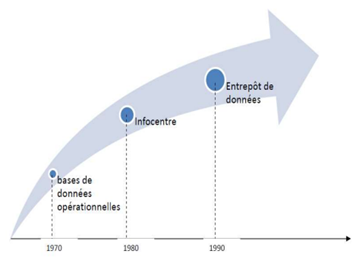
\includegraphics[]{evolutionDB}
	\end{center}
	\caption{Evolution des bases de donn\'ees d\'ecisionnelles}
	\label{Evolution des bases de donn�es d�cisionnelles}
\end{figure}
Le stockage en entrep�ts des donn�es a commenc� � la fin des ann�es 1980 lorsque Paul Murphy et Barry Devlin, employ�s d�IBM, a mis au point le Business Data Warehouse.\\
Cependant, le vrai concept a �t� donn� par Inmon Bill. Il �tait consid�r� comme le p�re de l�entrep�t de donn�es. Il avait �crit sur une vari�t� de sujets concernant la construction, l�utilisation et l�entretien de l�entrep�t et de l�usine d�information corporative.\\
\subsection{Mod\'elisation de donn\'ees d�un DW}
La mod\'elisation dimensionnelle d�un DW s�appuie sur les deux concepts suivants :

\subsubsection{Concepts}
\begin{itemize}
	\item \textbf{Concept de fait}: Les tables de fait contiennent les donn�es que l�on souhaite voir dans des rapports d�analyse. Une table de faits se pr�sente sous la forme d�un ensemble de colonnes stockant des valeurs dites mesures, et des cl�s �trang�res (identifiants) qui sont g�n�ralement les cl�s primaires associ�es aux tables de dimensions.
	\item \textbf{Concept de dimension}: Les tables de dimension sont les tables qui raccompagnent une table de faits, elles contiennent les descriptions textuelles de l�activit�. Une table de dimension est constitu�e de nombreuses colonnes qui d�crivent une ligne. C�est gr�ce � cette table que l�entrep�t de donn�es peut �tre compr�hensible et utilisable\cite{ref6}.  
\end{itemize}
\begin{figure}[!h]
	\begin{center}
		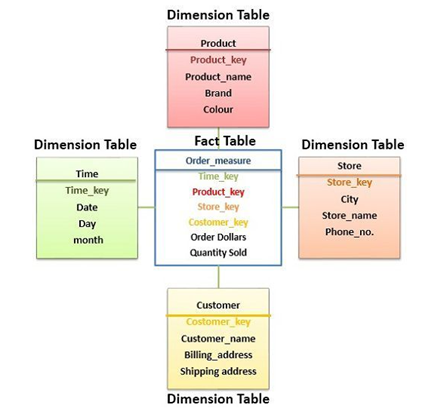
\includegraphics[]{archEtoileBI}
	\end{center}
	\caption{Architecture en \'etoile qui illustre le concept de fait et le concept de dimension}
	\label{Architecture en \'etoile qui illustre le concept de fait et le concept de dimension}
\end{figure}

Le tableau suivant r�sume les diff�rences entre les tables de faits et les tables de dimensions au niveau des donn�es\cite{ref7}:
\begin{figure}[!h]
	\begin{center}
		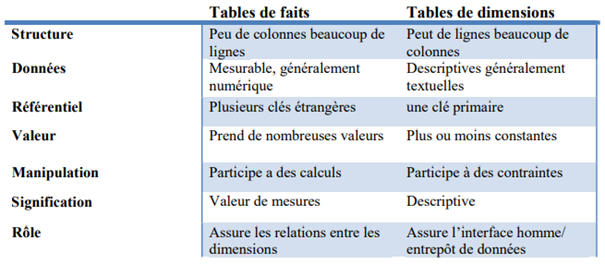
\includegraphics[]{tableFait}
	\end{center}
	\caption{Tableau comparatif entre les tables de faits et les tables de dimensions}
	\label{Tableau comparatif entre les tables de faits et les tables de dimensions}
\end{figure}
\subsubsection{Diff�rents mod�les de la mod�lisation dimensionnelle}
Principalement, les trois mod�les, couramment employ�s pour la mod�lisation dimensionnelle sont : 
\textbf{Mod�le en �toile}\\
Ce mod�le tire son nom de sa configuration, en effet il se forme d�un objet central qui est la table des faits reli�e � un ensemble de tables de dimensions. La force de ce type de mod�lisation est sa lisibilit� et sa performance. Pr�sent� dans le sch�ma ci-dessous :
\begin{figure}[!h]
	\begin{center}
		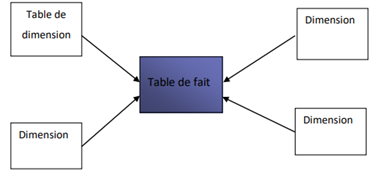
\includegraphics[]{modelisationEtoile}
	\end{center}
	\caption{Mod\'elisation en \'etoile}
	\label{Mod\'elisation en \'etoile}
\end{figure}

\textbf{Mod�le en flocon}\\
Identique au mod�le en �toile, sauf que ses branches sont �clat�es en hi�rarchies. Cette mod�lisation est g�n�ralement justifi�e par l��conomie d�espace de stockage, cependant elle peut s�av�rer moins compr�hensible pour l�utilisateur final et tr�s co�teuse en termes de performances.
\begin{figure}[!h]
	\begin{center}
		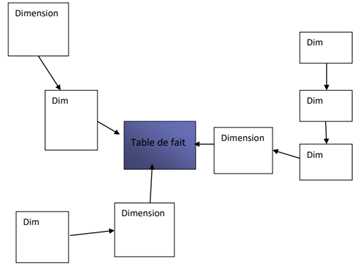
\includegraphics[]{modelFlocons}
	\end{center}
	\caption{Mod\'elisation en flocons}
	\label{Mod\'elisation en flocons}
\end{figure}

\textbf{Mod�le en constellation}\\
Ce n�est rien d�autre que plusieurs mod�les en �toiles li�s entre eux par des dimensions en commun.
\begin{figure}[!h]
	\begin{center}
		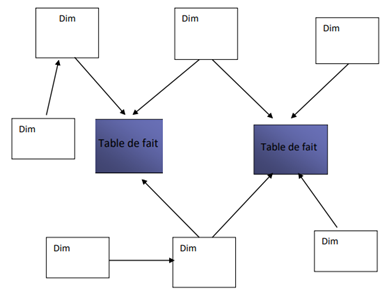
\includegraphics[]{modelConstellation}
	\end{center}
	\caption{Mod�lisation en constellation}
	\label{Mod�lisation en constellation}
\end{figure}

\subsection{Concept OLAP}
C�est une cat�gorie de logiciels ax�s sur l�exploration et l�analyse rapide des donn�es selon une approche multidimensionnelle � plusieurs niveaux d�agr�gation. 

Le noyau d�un syst�me OLAP est son serveur. Ces serveurs sont class�s en trois architectures syst�mes qui peuvent �tre distingu�es comme suit :

\begin{itemize}
	\item Les syst�mes � architecture MOLAP �Multidimentional On-line Analytical Processing� 
    \item Les syst�mes � architecture ROLAP �Relationnel On-line Analytical Processing� 
    \item Les syst�mes � architecture HOLAP �Hybride On-line Analytical Processing\cite{ref7}�\
\end{itemize}

\begin{figure}[!h]
	\begin{center}
		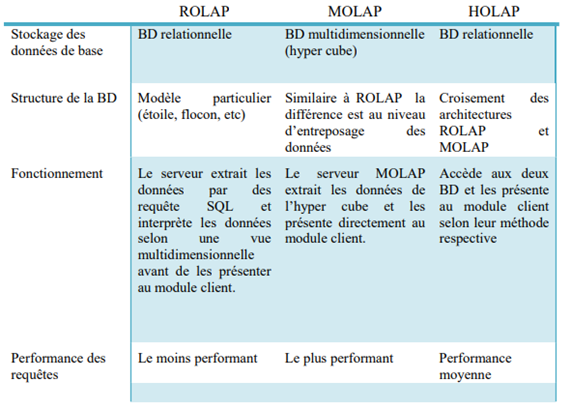
\includegraphics[]{comparatifArch}
	\end{center}
	\caption{Tableau comparatif des diff�rentes architectures OLAP}
	\label{Tableau comparatif des diff�rentes architectures OLAP}
\end{figure}

\subsection{Architecture et composants d�un syst�me BI}
Apr�s avoir d�fini la BI, on va d�couvrir ses composants et expliquer comment �a fonctionne les uns avec les autres. Le sch�ma suivant illustre l�architecture et les composants principaux d'un syst�me BI\cite{ref7} :


\begin{figure}[!h]
	\begin{center}
		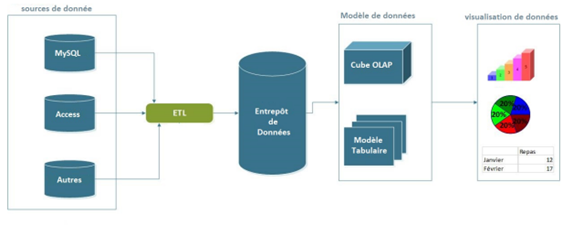
\includegraphics[]{archSysBI}
	\end{center}
	\caption{vue d'ensemble de l'architecture d'un systeme BI}
	\label{vue d'ensemble de l'architecture d'un systeme BI}
\end{figure}

L'architecture pr�sent�e dans la figure ci-dessus contient les composants les plus courants trouv�s dans la plupart des syst�mes de BI, car l'architecture de ses composants peut varier en fonction de l'outil, de l'environnement, etc. Chacun de ces composants seront discut�s plus en d�tail dans les sections qui suivent.

\subsubsection{Sources de donn�es}
Les sources de donn�es sont souvent diverses et vari�es on peut citer par exemple : les bases de donn�es relationnelles (MySQL, Oracle, SQL Server), les fichiers plats Excel, XML, les services web� etc. On ne peut pas construire un syst�me BI, sans source de donn�es.

\subsubsection{ETL}
Les sources de donn�es sont souvent diverses et vari�es on peut citer par exemple : les bases de donn�es relationnelles (MySQL, Oracle, SQL Server), les fichiers plats Excel, XML, les services web� etc. On ne peut pas construire un syst�me BI, sans source de donn�es.

\subsubsection{Entrep�t de donn�es}
Consid�r� comme �tant le c�ur du syst�me vu son importance, il sert � conserver toutes les donn�es de l�entreprise provenant de ses diff�rents services, dans le but de faciliter l�analyse des donn�es et le Reporting.

\subsubsection{Mod�le de donn�es}
Un Entrep�t de donn�es est con�u pour �tre la source d'analyse et de rapports, de sorte qu'il soit plus rapide que les syst�mes op�rationnels pour la production de rapports. Cependant, il n�est pas aussi rapide qu�il pr�tend, pour pouvoir couvrir tous les besoins, puisque lui-m�me est une base de donn�es relationnelle qui est d�finie avec un ensemble de contraintes qui r�duisent le temps de r�ponse d'une requ�te. L'exigence d'un traitement plus rapide en ayant un temps de r�ponse plus faible d'une part, et avoir des informations agr�g�es d�autre part, entraine donc la cr�ation d'une autre couche dans les syst�mes de BI. Cette couche, appel� Mod�le de donn�es, contient un mod�le de donn�es bas� sur des fichiers ou bas� sur la m�moire vive, afin de produire rapidement les r�ponses aux requ�tes pour l��dition des rapports\ref{ref7}.\\
Le \textbf{Mod�le de donn�es} s�appuie sur deux technologies : \textbf{Cube OLAP} et le mod�le en m�moire de tableau (\textbf{Mod�le tabulaire}).\\
Le \textbf{Cube OLAP} est un stockage de donn�es bas� sur un fichier qui charge les donn�es � partir d'un entrep�t de donn�es dans un mod�le de cube. Le cube contient des informations descriptives telles que les dimensions (par exemple, Etudiant et Parcours) et des cellules (par exemple, des faits et des mesures, telles que FactResultat et mesure les Admis).\\
Le \textdf{Mod�le tabulaire} est bas� sur un nouveau moteur en m�moire pour les tables. Le moteur en m�moire charge toutes les donn�es rang�es de tables dans la m�moire et r�pond � des questions directement � partir de la m�moire. C'est tr�s rapide en termes de temps de r�ponse.

\subsubsection{Visualisation de donn�es}
L'interface d'un syst�me BI\ref{ref7} est la visualisation de donn�es. En d'autres termes, la visualisation de donn�es est la partie du syst�me de BI que les utilisateurs peuvent voir. Il existe diff�rentes m�thodes pour la visualisation d'informations, tels que des tableaux de bord strat�giques et tactiques, indicateurs cl�s de performance ou Key performance Indicators (KPI), des rapports consolid�s.\\
C�est donc la partie qui int�resse le plus les d�cideurs d�une entreprise. De ce fait, il existe un grand nombre d�outils de visualisation de rapport sur le march�, telle que \textbf{SharePoint}, \textbf{PowerBI}, \textbf{IDashBoards}, etc.

\section{Solutions BI pr�sentes sur le march�}
De nombreux fournisseurs de solutions BI tentent de convaincre les clients des performances de leurs applications. Cependant, ces solutions de BI peuvent ne pas convenir � diff�rents environnements commerciaux. Dans la liste ci-dessous, vous pouvez voir les principaux fournisseurs de BI sur le march�. Destin�s principalement aux entreprises et aux soci�t�s, ces produits comprennent une suite compl�te d'applications, de bases de donn�es, d'outils d'int�gration et de visualisation.
\begin{itemize}
	\item IBM Cognost 
    \item SAP Business Objects
    \item Pantaho BI 
    \item SpagoBI 
    \item JasperSoft 
    \item SAS BI 
    \item Oracle BI
    \item Microsoft BI
\end{itemize}

\subsection{Environnement logiciel choisi}
Pour aboutir notre projet, nous avons d� employer un certain nombre d�outils et logiciels :
\begin{itemize}
	\item  \textbf{Microsoft Business Intelligence} :\\
Microsoft a montr� un int�r�t marqu� pour la prise de d�cision ces derni�res ann�es, l'entreprise ciblant un segment significatif du march�, et avec les solutions qu'il propose, on peut dire qu'il est trajectoire correcte. La plate-forme Microsoft est livr�e avec une vari�t� d'outils qui vous permettent d'effectuer des performances �lev�es tout au long du processus d�cisionnel. Nous citons :
	\begin{itemize}
		\item SQL Server Int�gration services (SSIS) ;
        \item SQL Server Analysis Services (SSAS) ;
        \item Microsoft Power BI
	\end{itemize}
	\item  \textbf{Syst�me de gestion de base de donn�es} :\\
SQL Server Management Studio (SSMS) est un outil pour acc�der, configurer, Administration, administration et d�veloppement de tous les composants de SQL Server. Associ�s SSMS Un ensemble d'outils graphiques pour habiliter les d�veloppeurs avec un puissant �diteur de scripts et les administrateurs de tous les niveaux peuvent acc�der � SQL Server.
   \begin{figure}[!h]
		\begin{center}
			
\includegraphics[]{sqlserver}
		\end{center}
		\caption{SQL Server logo}
		\label{SQL Server logo}
   \end{figure}
   \item \textbf{SSDT pour Visual Studio 2017}: \\
   \begin{figure}[!h]
		\begin{center}
			
\includegraphics[]{ssdt}
		\end{center}
		\caption{Visual Studio logo}
		\label{Visual Studio logo}
   \end{figure}
   SSDT est l�abr�viation de Microsoft SQL Server Data Tools, c�est un outil de d�veloppement moderne et un compl�ment � Visual Studio qui permet de d�velopper un projet BI complet avec ces diff�rentes phases.\\
Avec SSDt nous allons utiliser SQL Server Integration Services (SSIS) comme une solution d�int�gration et de transformation des donn�es et SQL Server Analysis Services (SSAS) comme une solution d�analyse des donn�es.
\item \textbf{Power BI Desktop}: \\
 Power BI, Business Intelligence d�velopp�e par Microsoft, est une suite d�outils d�informatique d�cisionnelle int�gr�e � Microsoft Office 365 pour :
 \begin{itemize}
 	\item Traiter, analyser des donn�es, provenant de multiples sources,
    \item Les transformer en informations exploitables, c.-�-d. les visualiser sous forme de rapports et tableaux de bord interactifs, en fonction de vos besoins descriptifs ou pr�dictifs,
    \item Les partager avec les �quipes concern�es, gr�ce � Office 365,
    \item Prendre des d�cisions tactiques ou strat�giques. \cite{ref10}
    \begin{figure}[!h]
		\begin{center}
			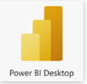
\includegraphics[]{logoBI}
		\end{center}
		\caption{Power BI Desktop logo}
		\label{Power BI Desktop logo}
   \end{figure}
 \end{itemize}
\end{itemize}

\section{D�marches et M�thodologies}
L�informatique d�cisionnelle est tout un concept, qui touche non seulement au c�t� technologique mais il met en valeur aussi l�importance du choix d�une m�thodologie de travail. Le choix d�une m�thodologie adapt�e � la soci�t� est indispensable pour la r�ussite du projet. Il faut notamment prendre en compte la vitesse d��volution des besoins et des priorit�s.\\

Bien que chaque projet de Business Intelligence (informatique d�cisionnelle) ou BI soit unique et r�ponde � des particularit�s techniques et processus d'ex�cution distincts, il est possible de d�finir quelques �tapes ou phases d'un projet de BI, ainsi qu'une s�rie de caract�ristiques communes dans presque tous les cas.

\begin{itemize}
	\item \textbf{�tape 1. D�finition des objectifs et besoins}\\
	Il s'agit l� d'une phase essentielle du processus et elle se caract�rise par la pr�cision, car, outre la d�finition des besoins et objectifs, il faut d�terminer quelles d�cisions concr�tes doivent �tre prises, quel type d'informations est n�cessaire et sur quelles variables l'analyse se basera-t-elle\cite{ref8}.
	\item \textbf{�tape 2. Choix de la m�thodologie}\\
	Toujours en fonction des objectifs et besoins du projet, il faut ensuite choisir la m�thodologie concr�te et les outils de BI � utiliser, ce qui implique aussi la formation et mise en place des �quipes de travail\cite{ref8}.
	\item \textbf{�tape 3. Mise en place du programme de travail}\\
	Il convient de d�finir, de mani�re d�taill�e, pr�cise et claire, toutes les actions � r�aliser, ainsi que l�infrastructure et les ressources n�cessaires pour englober la m�thodologie d'analyse de donn�es choisie ainsi que les d�lais d'ex�cution du projet de Business Intelligence\cite{ref8}.
	\item \textbf{�tape 4. Actions de pr�sentation}\\
	L'�tape suivante consiste � �laborer et pr�senter des rapports, reports, tableaux de bord, diagrammes de flux et infographies, de fa�on tr�s visuelle, claire et sch�matique, afin de faciliter le travail des professionnels charg�s de prendre des d�cisions\ref{ref8}.
	\item \textbf{�tape 5. Ex�cution du syst�me, formation et de support}\\
	L'ex�cution d'un processus de Business Intelligence ne sera utile que si les informations, correctement analys�es, arrivent aux personnes ayant la capacit� de d�cider dans le support et avec les outils ad�quats\cite{ref8}.
\end{itemize}

\subsection{M�thodologie de travail}
Pour r�aliser et r�ussir un projet, il est important de suivre une m�thodologie adapt�e. Il s'agit d'un outil qui vous aide � accomplir votre projet �tape par �tape, de la planification � la mise en �uvre, dans un souci d'efficacit� et rentabilit�\cite{ref9}.\\
Il existe de nombreuses approches de la gestion de projet et faire le bon choix n'est pas toujours facile car il n'y a pas d'approche unique pour un projet, une entreprise ou une industrie. Une m�thode fonctionne pour une situation mais pas pour une autre, et parfois vous devez combiner diff�rents �l�ments de plusieurs m�thodes pour cr�er la v�tre\\.
Choisir la bonne m�thodologie de gestion de projet est donc une �tape indispensable pour r�ussir votre projet. Optez pour une m�thode qui valorise les objectifs de votre projet et les points forts de votre �quipe. Vous pouvez �galement cr�er une m�thodologie hybride qui assemble des �l�ments de diff�rentes m�thodologies. Traditionnelle, agile ou autres, l'essentiel est que vous et votre �quipe trouviez la m�thode de travail qui vous convienne le mieux.\\

\subsection{Approches de mod�lisation BI Adopt�}
Pour faire une  conception d'entrep�t de donn�es (DWH), deux des approches d'entrep�t de donn�es les plus largement discut�es et expliqu�es sont les m�thodologies Inmon et Kimball. Pendant des ann�es, les gens ont d�battu de l'approche d'entrep�t de donn�es la meilleure et la plus efficace pour les entreprises. Cependant, il n'y a toujours pas de r�ponse d�finitive car les deux m�thodes ont leurs avantages et leurs inconv�nients.

\subsubsection{Inmon : de l�entrep�t aux magasins}
Dans les ann�es 1990, William Inmon propose une vision descendante de la structuration de la donn�e de l�entreprise, dite ``top-down``.\\

L�entrep�t de donn�e a pour r�le de rassembler toutes les donn�es de l�entreprise, et les magasins de donn�es sont alors des sous-parties issues de cet entrep�t.
\begin{figure}[!h]
	\begin{center}
		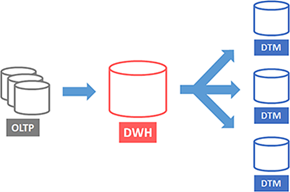
\includegraphics[]{topDown}
	\end{center}
	\caption{L�approche top-down}
	\label{L�approche top-down}
\end{figure}
\subsubsection{Kimball : des magasins � l�entrep�t}
Ralph Kimball propose une vision radicalement diff�rente, ascendante, de la structuration de la donn�e, dite ``bottom-up``.\\
Les besoins de l�entreprise sont mod�lis�s dans les magasins de donn�es, l�entrep�t de donn�es n�est par la suite qu�une simple union de ses magasins de donn�es.

\begin{figure}[!h]
	\begin{center}
		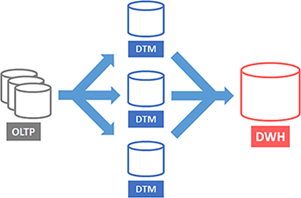
\includegraphics[]{bottomUp}
	\end{center}
	\caption{Approche bottom\-up}
	\label{Approche bottom\-up}
\end{figure}

D�apr�s le cycle de vie de notre projet on a utilis� l�approche de Ralph KIMBALL qui nous permet de mettre en place une conception appuy�e sur des phases de fonctionnement clairement �tablies et des points de v�rification pr�d�finis, avec un avantage du sch�ma en �toile est que la plupart des op�rateurs de donn�es peuvent facilement le comprendre en raison de sa structure d�normalis�e, ce qui simplifie les requ�tes et l'analyse.

\section{Conclusion}
Dans ce chapitre, j�ai commenc� par une pr�sentation des concepts de base des syst�mes d�cisionnels (BI) et leurs divergences avec les syst�mes transactionnels. Par la suite, on a d�taill� l�architecture globale d�un cycle BI et en particulier ses diff�rents composants. Puis on s�est int�ress� aux diff�rentes solutions BI pr�sentes dans le march�. Pour en conclure, j�ai pr�sent� les deux m�thodologies celle de  Inmon et l�autre de Kimball (utilis� vu les moyens, la cible et la dur�e de notre stage).
\chapter{Conception et D�veloppement de l�ETL}
\section{Introduction}
L��tude de l�existant nous a permis de d�celer les objectifs et les attentes de l�ISET et elle nous a fourni une vision claire de ce que nous allons aborder dans ce troisi�me chapitre. Dans ce chapitre, on va exposer l�architecture sur laquelle sera fond� notre syst�me ce qui nous permettra de r�aliser respectivement la mod�lisation, la conception et finalement l�impl�mentation du Data Warehouse.\\
Les �tapes de l'entrep�t de donn�es doivent �tre con�ues de mani�re que les bonnes informations soient facilement accessibles au bon moment. L'architecture choisie est repr�sent�e par un mod�le logique sous forme de 4 couches.

\begin{itemize}
	\item Couche source de donn�es;
    \item Couche de pr�paration de donn�es (Data StagingDataSource);
    \item Couche de stockage de donn�es (DWH);
    \item Couche de pr�sentation et restitution de donn�es;
\end{itemize}

On va d�tailler ces 4 couches selon notre sujet comme suit :

\section{Couche source de donn�es}
Cette couche repr�sente les diff�rentes sources de donn�es dans diff�rents formats du syst�me d'exploitation qui sont pr�tes � �tre introduites dans l'entrep�t de donn�es. Dans notre cas (sous forme de fichiers Excel)\\
Pour r�aliser cette �tape, il a fallu extraire les relations existantes entre les tables des bases de donn�es, pour cela j�ai utilis� l�outils : MySQL Workbench pour faire les liaisons entre les tables et fournir une base de donn�es plus au moins claire qui nous a donn� le diagramme suivant :

\begin{figure}[!h]
	\begin{center}
		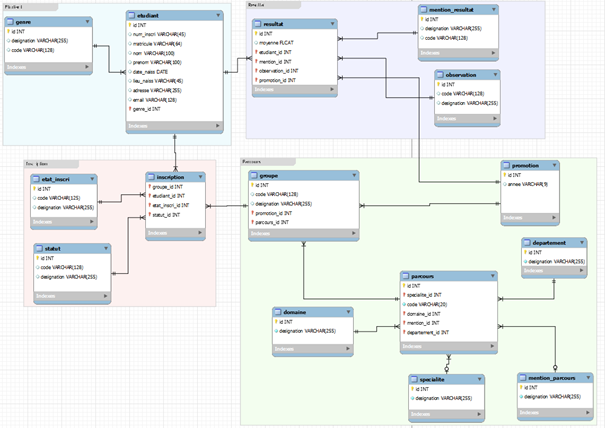
\includegraphics[]{modelRelationnel}
	\end{center}
	\caption{Mod�le Relationnel de la Base de donn�es Partie relation entre les tables}
	\label{Mod�le Relationnel de la Base de donn�es Partie relation entre les tables}
\end{figure}

\section{Couche de pr�paration de donn�es (StagingDataSource)}
Cette couche est la couche de pr�paration des donn�es (Data Staging), principalement pour une extraction rapide de Donn�es provenant de sources d'information. Apr�s avoir charg� les donn�es Dans StagingDataSource, l'�tape de transformation entre en jeux (suppression redondance des donn�es, filtrage des donn�es erron�es) et Validez les donn�es avant de les transf�rer vers DWH.\\
On peut nommer cette couche par la partie \begin{bf}ETL\end{bf} (Extract-Tansform-LOAD).\\

\subsubsection{Extract: Extraction de donn�es brutes}
La premi�re �tape et la pr�paration de la base de donn�es Staging avec la cr�ation de la table \begin{bf}audit_logs\end{bf} et les \begin{bf}fonctions\end{bf}

\begin{figure}[!h]
	\begin{center}
		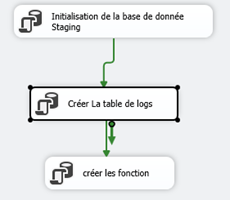
\includegraphics[]{auditLogs}
	\end{center}
	\caption{Pr�paration au Staging}
	\label{Pr�paration au Staging}
\end{figure}

\begin{itemize}
	\item \begin{bf}Audit_logs\end{bf} appel� aussi journal d�audit est essentiellement un enregistrement des �v�nements et des modifications. Il nous permet de noter tous les changements au sein de notre travail, fournissant un historique complet des op�rations r�alis�. 
	
	\begin{figure}[!h]
		\begin{center}
			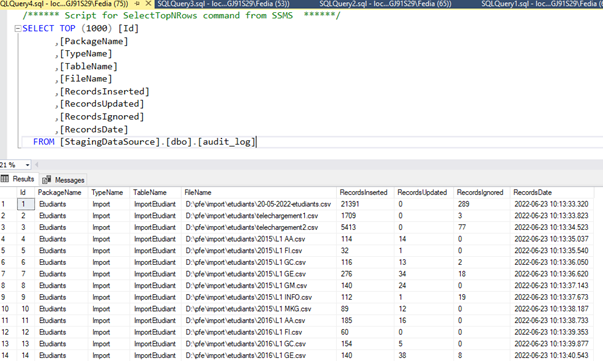
\includegraphics[]{operation1}
		\end{center}
		\caption{affichage de l�historique des op�rations}
		\label{affichage de l�historique des op�rations}
	\end{figure}
	
	\item \begin{bf}Les fonctions\end{bf} sont cr��es pour nous aider dans la phase de nettoyage et transformation des donn�es.
	\newpage
	\begin{figure}[!h]
		\begin{center}
			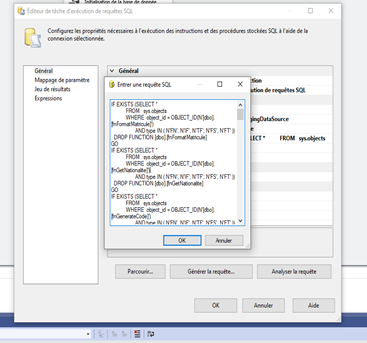
\includegraphics[]{creationFonction}
		\end{center}
		\caption{cr�ation des fonctions}
		\label{cr�ation des fonctions}
	\end{figure}
	
	\begin{figure}[!h]
		\begin{center}
			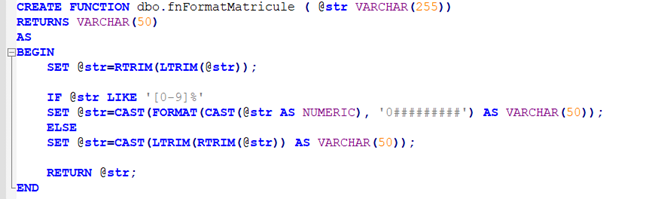
\includegraphics[width=450pt,height=250pt]{creationdbo}
		\end{center}
		\caption{cr�ation dbo.fnFormatMatricule}
		\label{cr�ation dbo.fnFormatMatricule}
	\end{figure}
	\newpage
	\begin{figure}[!h]
		\begin{center}
			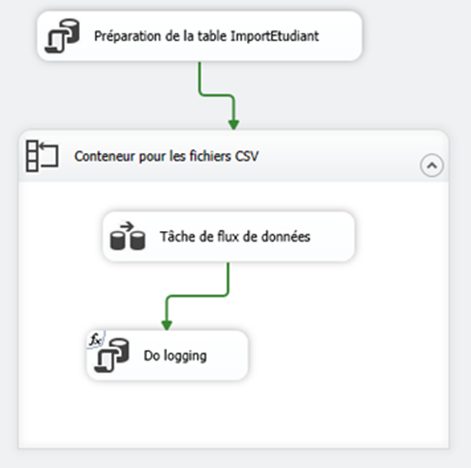
\includegraphics[width=390pt, height=290pt]{chargementTable}
		\end{center}
		\caption{Chargement de la table ImportEtudiant}
		\label{Chargement de la table ImportEtudiant}
	\end{figure}
	
	\begin{figure}[!h]
		\begin{center}
			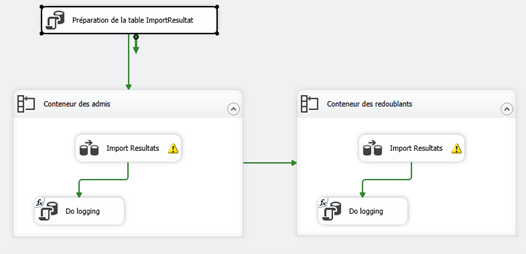
\includegraphics[]{chargementTable2}
		\end{center}
		\caption{Chargement de la table ImportResultat}
		\label{Chargement de la table ImportResultat}
	\end{figure}
	\newpage
	\begin{figure}[!h]
		\begin{center}
			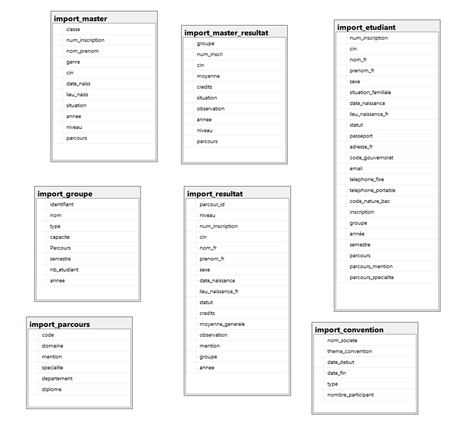
\includegraphics[]{importFichier}
		\end{center}
		\caption{Mod�le Relationnel de la Base de donn�es Partie ImportFichier}
		\label{Mod�le Relationnel de la Base de donn�es Partie ImportFichier}
	\end{figure}
	
	Le mod�le ci-dessus est le r�sultat du processus d�import des fichiers Excel qui sont transform� en format CSV import� de SALIMA et du logiciel con�us pour les �tudiants de mast�re et un autre fichier Excel pour les conventions. Ce mod�le se compose de 7 tables diff�rentes, qui sont : 
	\begin{itemize}
		\item \begin{bf}Table ImportMaster\end{bf}: Contient les diff�rentes informations sur un �tudiants mast�re (cin, num�ro inscription, genre, nom pr�nom, ann�e, niveau, parcours,etc);
		\item \begin{bf}Table ImportMasterResultat\end{bf}: Contient les diff�rentes informations concernant r�sultat Mast�re (groupe, cin, num�ro inscription, moyenne, cr�dit, observation, ann�e, niveau, parcours, situation);
		\item \begin{bf}Table ImportEtudiant\end{bf}: Contient les diff�rentes informations concernant tous les �tudiants ( cin, num�ro inscription, nom, pr�nom, �mail, statut, �tat, ann�e, semestre, parcours,�etc);
		\item \begin{bf}Table ImportGroupe\end{bf}: Contient les diff�rents groupes existant � l�ISET( nom groupe, type, capacit�, parcours, semestre, ann�e);
		\item \begin{bf}Table ImportResultat\end{bf}: Contient les diff�rentes informations concernant r�sultat des �tudiants( cin, num�ro inscription, nom, pr�nom, moyenne g�n�ral, observation, mention, ann�e,�etc);
		\item \begin{bf}Table ImportConvention\end{bf}: Contient les diff�rentes informations concernant les conventions( nom soci�t�, th�me convention, type convention, date d�but, date fin, nombre participant);
		\item \begin{bf}Table ImportParcours\end{bf}: Contient les diff�rentes informations concernant les parcours existants( domaine, sp�cialit�, d�partement, dipl�me);
	\end{itemize}
\end{itemize}

\subsubsection{Tansform : Transformation, homog�n�isation et nettoyage de ces donn�es}

\begin{figure}[!h]
	\begin{center}
		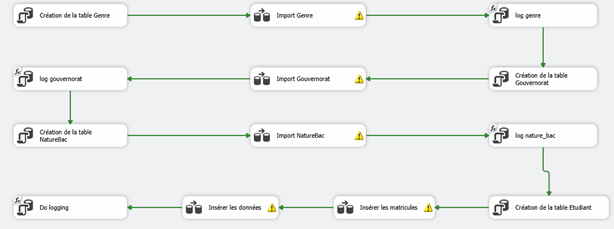
\includegraphics[]{transformationEtNettoyage}
	\end{center}
	\caption{Transformation et nettoyages de donn�es pour la cr�ation de la table Etudiants}
	\label{Transformation et nettoyages de donn�es pour la cr�ation de la table Etudiants}
\end{figure}

\begin{figure}[!h]
	\begin{center}
		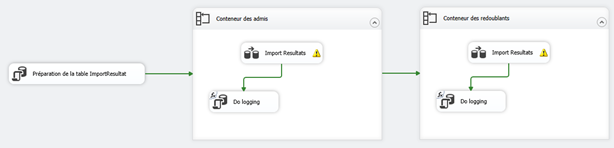
\includegraphics[]{transformationEtNettoyage2}
	\end{center}
	\caption{Transformation et nettoyages de donn�es pour la cr�ation de la table Resultat}
	\label{Transformation et nettoyages de donn�es pour la cr�ation de la table Resultat}
\end{figure}

\begin{figure}[!h]
	\begin{center}
		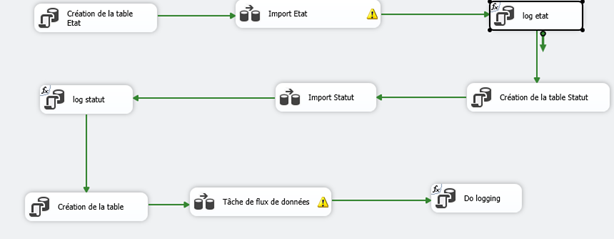
\includegraphics[]{transformationEtNettoyage3}
	\end{center}
	\caption{Transformation et nettoyages de donn�es pour la cr�ation de la table Inscription}
	\label{Transformation et nettoyages de donn�es pour la cr�ation de la table Inscription}
\end{figure}


\begin{figure}[!h]
	\begin{center}
		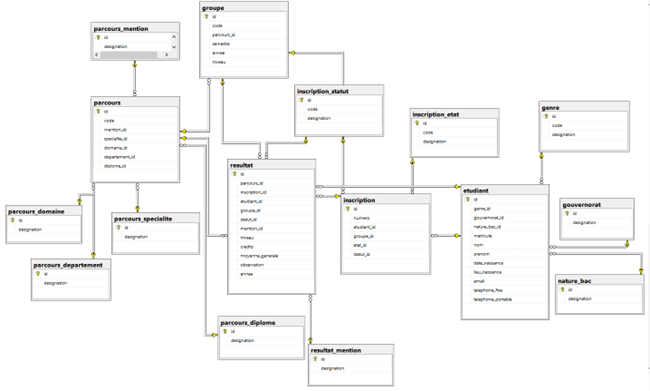
\includegraphics[]{modelRelationnelEtudiant}
	\end{center}
	\caption{Mod�le Relationnel de la Base de donn�es Partie Etudiant}
	\label{Mod�le Relationnel de la Base de donn�es Partie Etudiant}
\end{figure}

\begin{figure}[!h]
	\begin{center}
		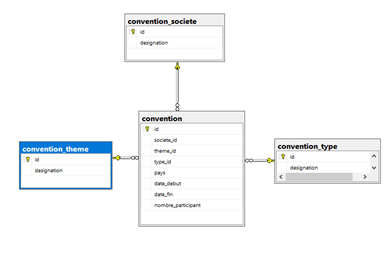
\includegraphics[]{modelRelationnelConevntion}
	\end{center}
	\caption{Mod�le Relationnel de la Base de donn�es Partie Convention}
	\label{Mod�le Relationnel de la Base de donn�es Partie Convention}
\end{figure}

Ces 2 mod�les ci-dessus est le r�sultat de la transformation des donn�es � partir des tables (\begin{bf}Table ImportMaster, Table ImportMasterResultat, Table ImportEtudiant, Table ImportGroupe , Table ImportResultat, Table ImportConvention, Table ImportParcours\end{bf}). Ce mod�le se compose de 20 tables diff�rentes, qui sont : 

\begin{itemize}
	\item Table Etudiant.
    \item Table Inscription.
    \item Table Parcours.
    \item Table Nature Bac.
    \item Table Genre.
    \item Table Gouvernorat.
    \item Table Inscription Etat.
    \item Table Inscription Statut.
    \item Table Groupe.
    \item Table R�sultat.
    \item Table D�partement.
    \item Table R�sultat Mention.
    \item Table parcours Dipl�me.
    \item Table parcours Sp�cialit�.
    \item Table parcours D�partement.
    \item Table parcours Domaine.
    \item Table convention.
    \item Table Convention Type.
    \item Table Convention Th�me.
    \item Table Convention Partenaire.
\end{itemize}

\section{Couche de stockage de donn�es (DWH)}
C�est la couche de l�alimentation de l�entrep�t de donn�es (DWH) pour stocker des informations analytiques et historiques qui seront utilis�es.\\
Apr�s la transformation et le nettoyage des donn�es et les stocker dans notre Staging on passe maintenant � l�alimentation des tables de fait et dimension et on a obtenu ce diagramme :

\begin{figure}[!h]
	\begin{center}
		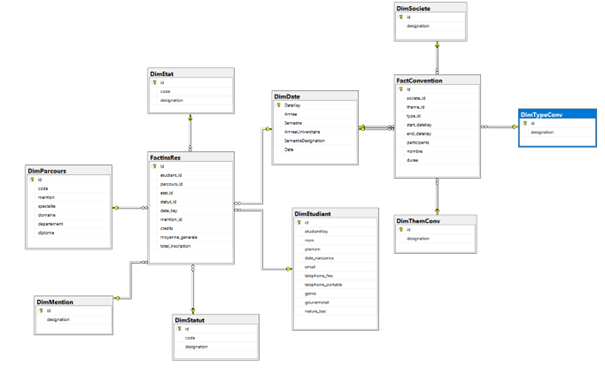
\includegraphics[]{modelEtoile}
	\end{center}
	\caption{Mod�le en �toile (DWH)}
	\label{Mod�le en �toile (DWH)}
\end{figure}

\section{Couche de pr�sentation et restitution de donn�es}
Cette couche fait r�f�rence aux informations qui parviennent � l'utilisateur final, telles que les rapports, gr�ce � cette couche, l'utilisateur pourra : 
\begin{itemize}
	\item Analyser les donn�es, notamment avec les outils de type OLAP pour les analyses multidimensionnelles
    \item Aide � la d�cision des d�cideurs en situation avec les tableaux de bord pr�sentant les indicateurs cl�s de l'activit�
    \item Transmettre l�efficacit� avec le Reporting.
\end{itemize}
Cette partie seras plus d�taill� dans le chapitre 4

	

\bibliographystyle{acm} % Le style est mis entre accolades.
\bibliography{reference} % mon fichier de base de donn�es s'appelle reference.bib
\addcontentsline{toc}{chapter}{Bibliographie et Netographie}

\begin{appendix}


\chapter{Annexes} \addcontentsline{toc}{chapter}{Annexes}
%\input{annexe.tex}


\end{appendix}

\end{document}

